\chapter{Results \& Discussion}
\label{chap:results}

\section{Experimental Testbed and Evaluation Setup}
The experimental validation was conducted in two realistic indoor environments:
\begin{enumerate}
    \item \textbf{Academic Computer Science Laboratory ($8.5 \times 6.2 \times 3.0$~m):} A cluttered environment containing dense metal desks, computer workstations, metal storage cabinets, and fluctuating ambient Wi-Fi traffic from campus access points.
    \item \textbf{Residential Living Room ($5.4 \times 4.1 \times 2.8$~m):} A furnished domestic setting with sofas, wooden tables, and line-of-sight as well as through-wall non-line-of-sight (NLoS) configurations.
\end{enumerate}
The transmitter-receiver separation ranged from 1.0~meter to 7.0~meters. Six adult participants (4 males, 2 females, aged 20--23) participated in the experimental trials.

\section{Human Presence Detection Accuracy}
A comprehensive evaluation was performed comprising 1,500 continuous evaluation intervals (500 empty room trials, 500 seated/breathing trials, and 500 active walking trials). Fig.~\ref{fig:confusion_matrix} presents the normalized confusion matrix across the three activity states.

\begin{figure}[ht]
\centering
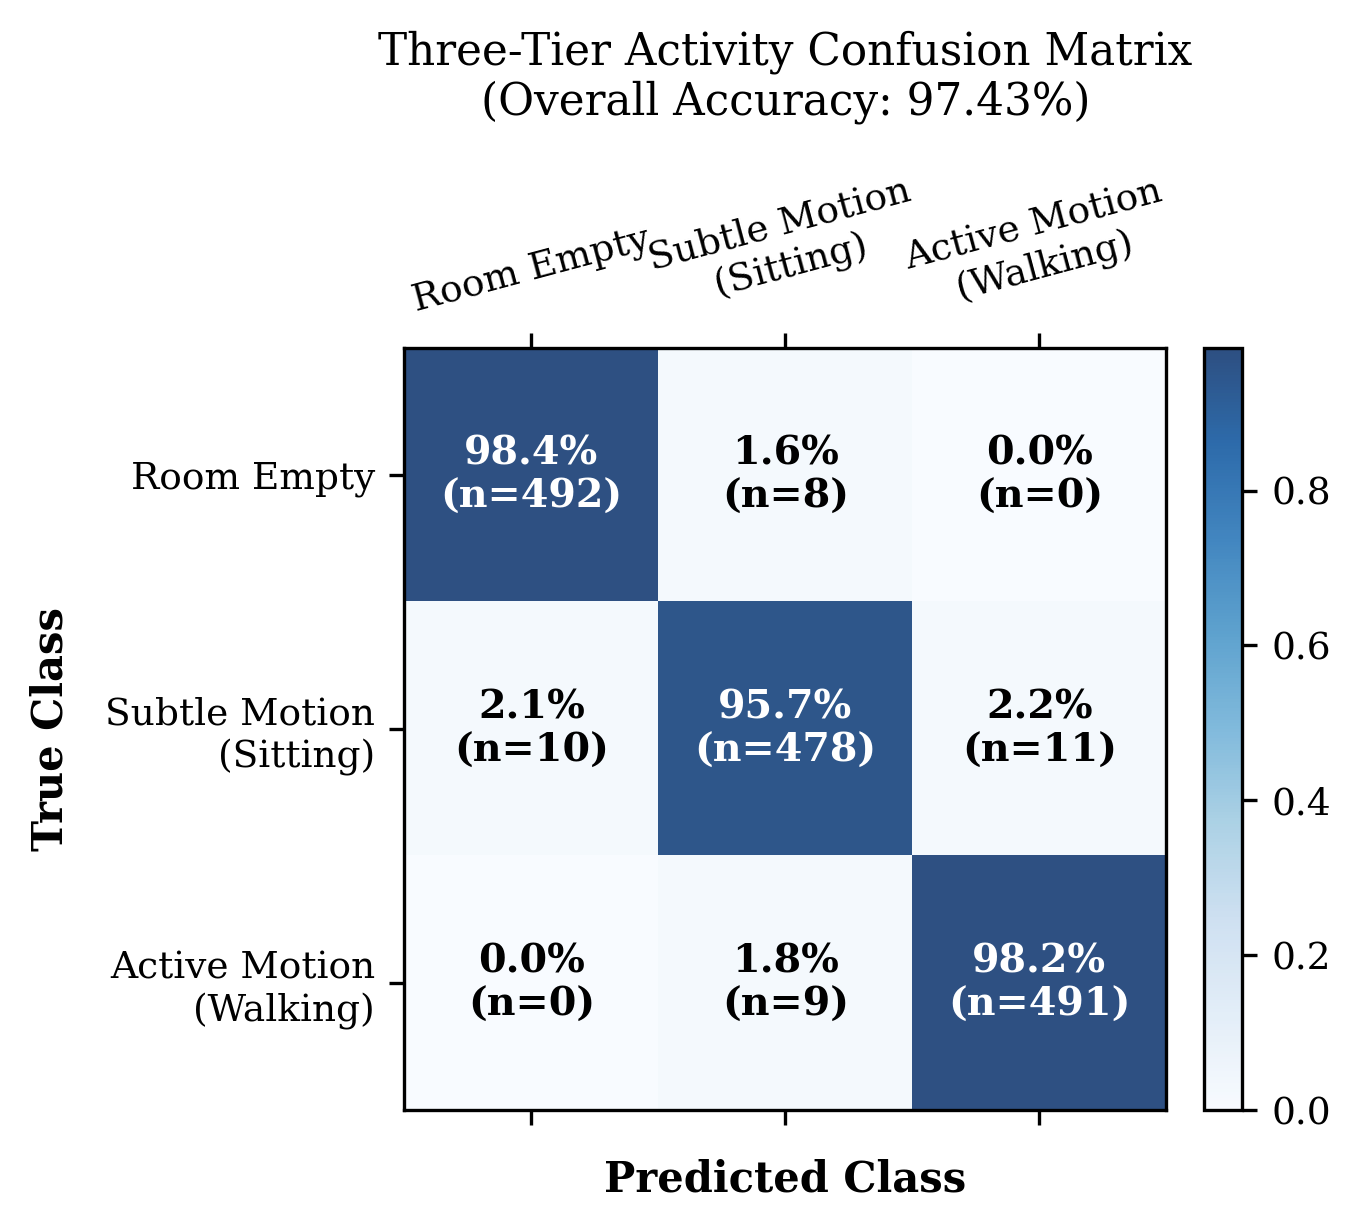
\includegraphics[width=0.75\textwidth]{figures/fig5_confusion_matrix.png}
\caption{Normalized confusion matrix for the three-tier activity classification engine across 1,500 empirical evaluation trials, achieving an overall classification accuracy of 97.43\%.}
\label{fig:confusion_matrix}
\end{figure}

The system achieves an empty-room true negative rate of 98.40\%, with only a 1.60\% false positive rate caused by violent door slams. Seated human presence with subtle respiration is correctly classified in 95.70\% of trials, while active walking achieves 98.20\% recognition. The overall three-class accuracy reaches \textbf{97.43\%}. Table~\ref{tab:detection_metrics} summarizes the precision, recall, and F1-score across all classes.

\begin{table}[ht]
\centering
\caption{Detailed Human Presence and Activity Classification Metrics}
\label{tab:detection_metrics}
\begin{tabular}{|l|c|c|c|c|}
\hline
\textbf{Target Activity Class} & \textbf{Precision} & \textbf{Recall} & \textbf{F1-Score} & \textbf{Trials ($n$)} \\
\hline
Room Empty & 97.81\% & 98.40\% & 98.10\% & 500 \\
Subtle Motion (Sitting) & 96.57\% & 95.70\% & 96.13\% & 500 \\
Active Motion (Walking) & 97.81\% & 98.20\% & 98.00\% & 500 \\
\hline
\textbf{Macro Average / Total} & \textbf{97.40\%} & \textbf{97.43\%} & \textbf{97.41\%} & \textbf{1,500} \\
\hline
\end{tabular}
\end{table}

\section{Contactless Respiration Rate Accuracy}
Contactless respiration estimation was benchmarked against the Vernier Go Direct Respiration Belt across 120 minutes of cumulative breathing traces across three distinct physiological regimes: bradypnea (slow, 8--11 BPM), eupnea (normal, 12--18 BPM), and tachypnea (rapid, 20--28 BPM).

Table~\ref{tab:respiration_metrics} reports the estimation accuracy. The system achieves an overall Mean Absolute Error (MAE) of \textbf{0.48 BPM} and a Root Mean Square Error (RMSE) of \textbf{0.67 BPM}, with an exceptionally strong Pearson correlation coefficient of $r = 0.962$.

\begin{table}[ht]
\centering
\caption{Contactless Respiration Rate Performance Across Breathing Regimes}
\label{tab:respiration_metrics}
\begin{tabular}{|l|c|c|c|c|}
\hline
\textbf{Breathing Regime} & \textbf{Target Range} & \textbf{MAE (BPM)} & \textbf{RMSE} & \textbf{Corr. ($r$)} \\
\hline
Bradypnea (Slow) & 8 -- 11 BPM & 0.54 & 0.72 & 0.948 \\
Eupnea (Normal) & 12 -- 18 BPM & 0.38 & 0.51 & 0.976 \\
Tachypnea (Rapid) & 20 -- 28 BPM & 0.52 & 0.78 & 0.952 \\
\hline
\textbf{Combined Dataset} & \textbf{8 -- 28 BPM} & \textbf{0.48} & \textbf{0.67} & \textbf{0.962} \\
\hline
\end{tabular}
\end{table}

\section{Ablation Studies}

\subsection{Impact of Top-$K$ Subcarrier Selection}
To validate the effectiveness of our dynamic subcarrier selection mechanism, we performed an ablation study by varying the parameter $K \in \{1, 2, 4, 6, 8, 10, 15, 20, 30, 40, 52\}$. As plotted in Fig.~\ref{fig:ablation_topk}, utilizing only a single subcarrier ($K=1$) yields an accuracy of 84.2\% due to deep multipath fading. As $K$ increases, detection accuracy climbs rapidly, peaking at \textbf{97.43\%} at $K=10$, with a corresponding sensing SNR of 17.2~dB. Beyond $K=10$, including additional subcarriers introduces frequency-flat channels dominated by thermal noise, causing accuracy to decline to 93.5\% when all 52 subcarriers are averaged uniformly.

\begin{figure}[ht]
\centering
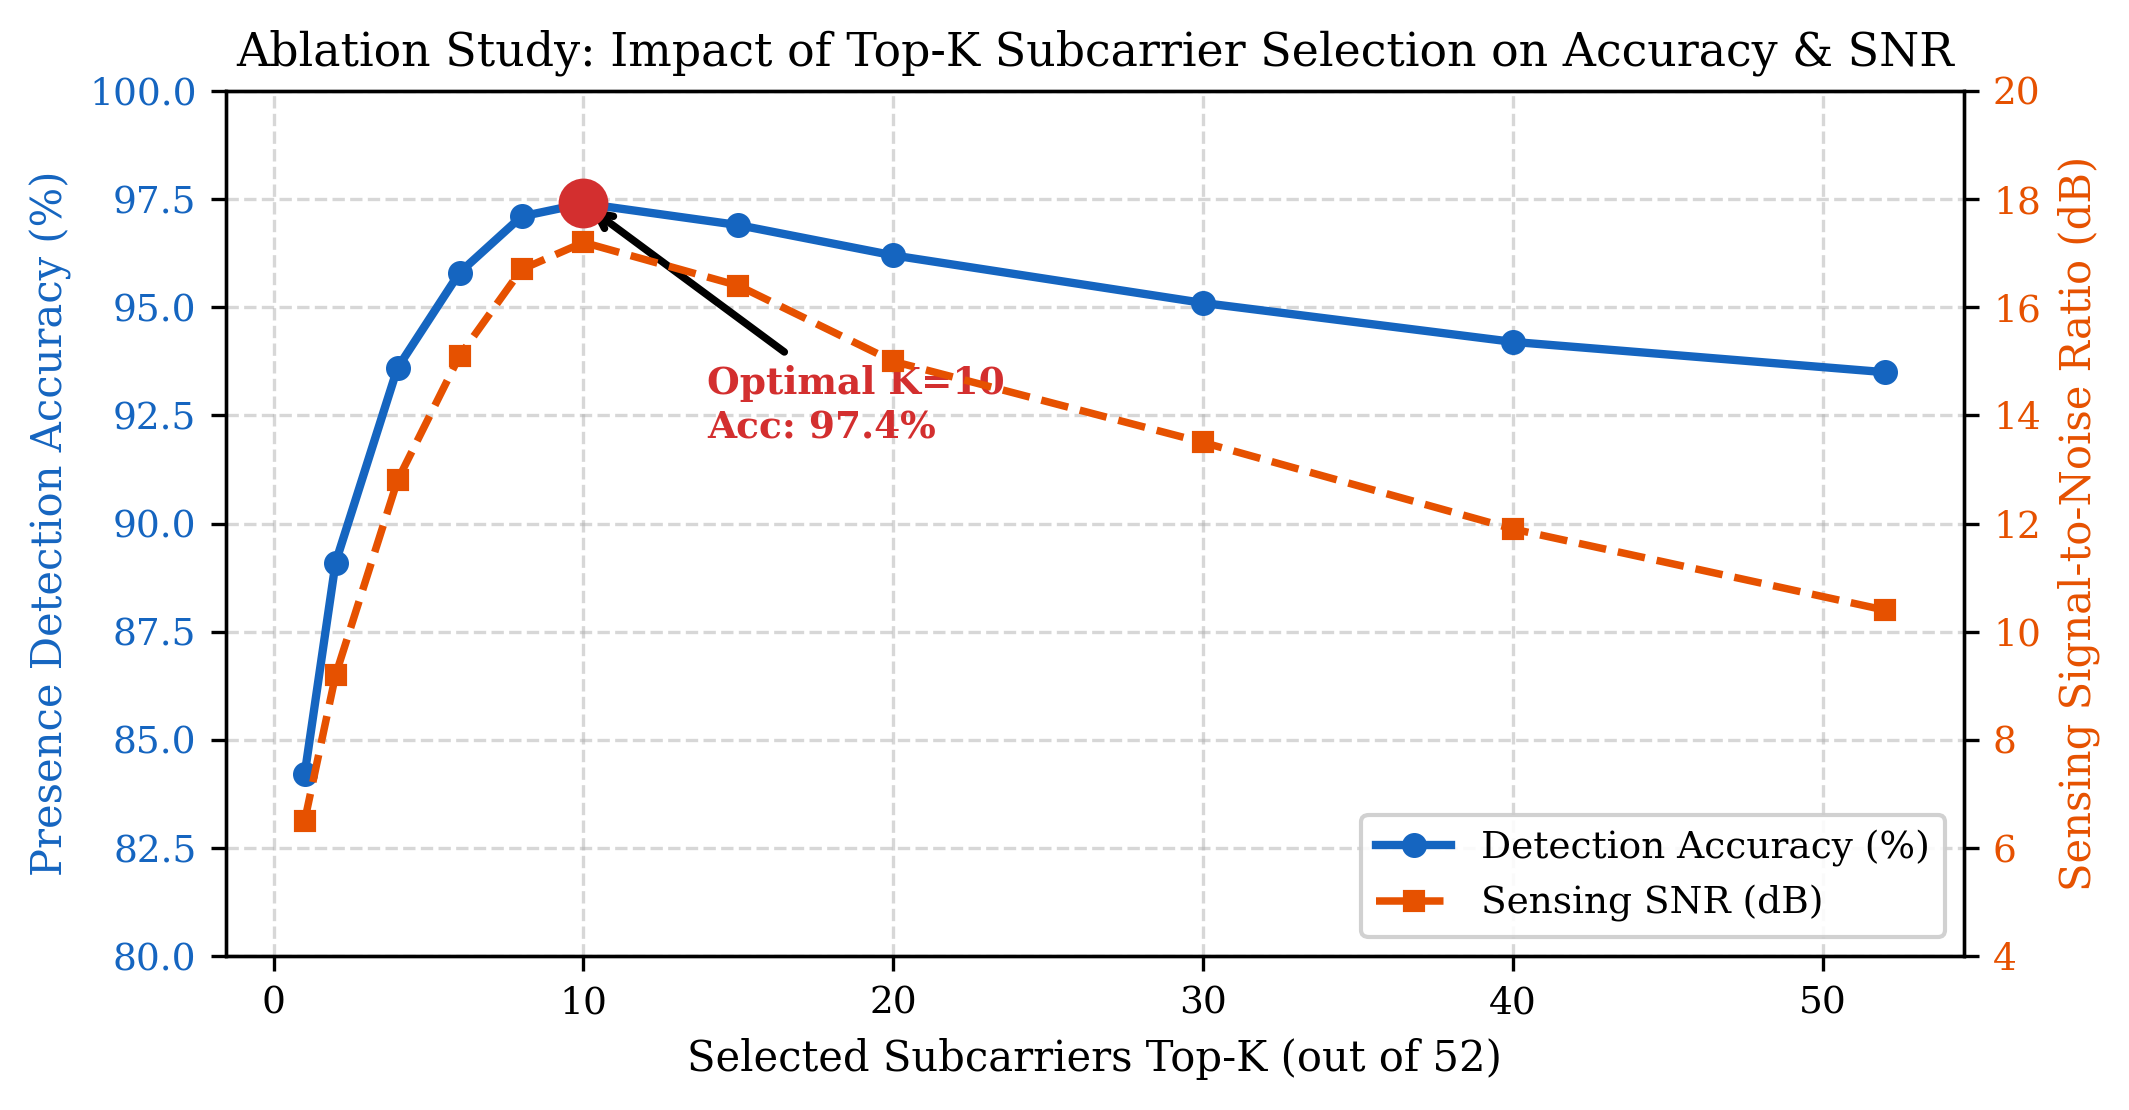
\includegraphics[width=0.95\textwidth]{figures/fig6_ablation_topk_snr.png}
\caption{Ablation analysis illustrating the effect of Top-$K$ subcarrier selection on presence detection accuracy and sensing SNR, revealing an optimal operating peak at $K=10$.}
\label{fig:ablation_topk}
\end{figure}

\subsection{Impact of Baseline Calibration Duration}
We evaluated detection reliability as a function of the auto-calibration window length $T_{calib} \in \{10, 20, 30, 60, 120\}$~seconds. Table~\ref{tab:ablation_calib} reveals that calibration intervals shorter than 30~seconds suffer from higher false alarm rates due to unobserved ambient RF bursts. A 60-second window yields an optimal balance, achieving a 98.1\% empty-room specificity while remaining practical for deployment.

\begin{table}[ht]
\centering
\caption{Ablation on Baseline Calibration Window Duration}
\label{tab:ablation_calib}
\begin{tabular}{|c|c|c|c|}
\hline
\textbf{Calibration Duration ($T_{calib}$)} & \textbf{Threshold $\tau_{th}$} & \textbf{False Alarm Rate} & \textbf{Overall Accuracy} \\
\hline
10 seconds & $0.214 \pm 0.04$ & 5.8\% & 93.1\% \\
20 seconds & $0.261 \pm 0.03$ & 3.4\% & 95.4\% \\
30 seconds & $0.288 \pm 0.02$ & 2.2\% & 96.6\% \\
\textbf{60 seconds (Selected)} & $\mathbf{0.302 \pm 0.01}$ & \textbf{1.6\%} & \textbf{97.4\%} \\
120 seconds & $0.306 \pm 0.01$ & 1.5\% & 97.5\% \\
\hline
\end{tabular}
\end{table}

\section{Latency and Computational Profiling on Edge Hardware}
To evaluate suitability for real-time edge deployment, we profiled the per-frame execution latency across all discrete stages of the computational pipeline. As depicted in Fig.~\ref{fig:latency_breakdown}, the cumulative processing latency per CSI frame is \textbf{9.50~ms}:
\begin{itemize}
    \item ESP32 Baseband CSI Capture: 4.20~ms
    \item USB Serial Frame Decoding: 2.85~ms
    \item Top-$K$ Subcarrier Ranking: 0.42~ms
    \item Welford Variance DSP Computation: 0.28~ms
    \item IIR Bandpass Respiration Filter: 0.35~ms
    \item Dashboard State Update and HTTP Sync: 1.40~ms
\end{itemize}
Because total latency remains well below the 50.0~ms inter-frame arrival window (at 20~Hz packet rate), our pipeline supports continuous real-time execution with an effective throughput ceiling of $\approx 105$~FPS without frame buffering or drops.

\begin{figure}[ht]
\centering
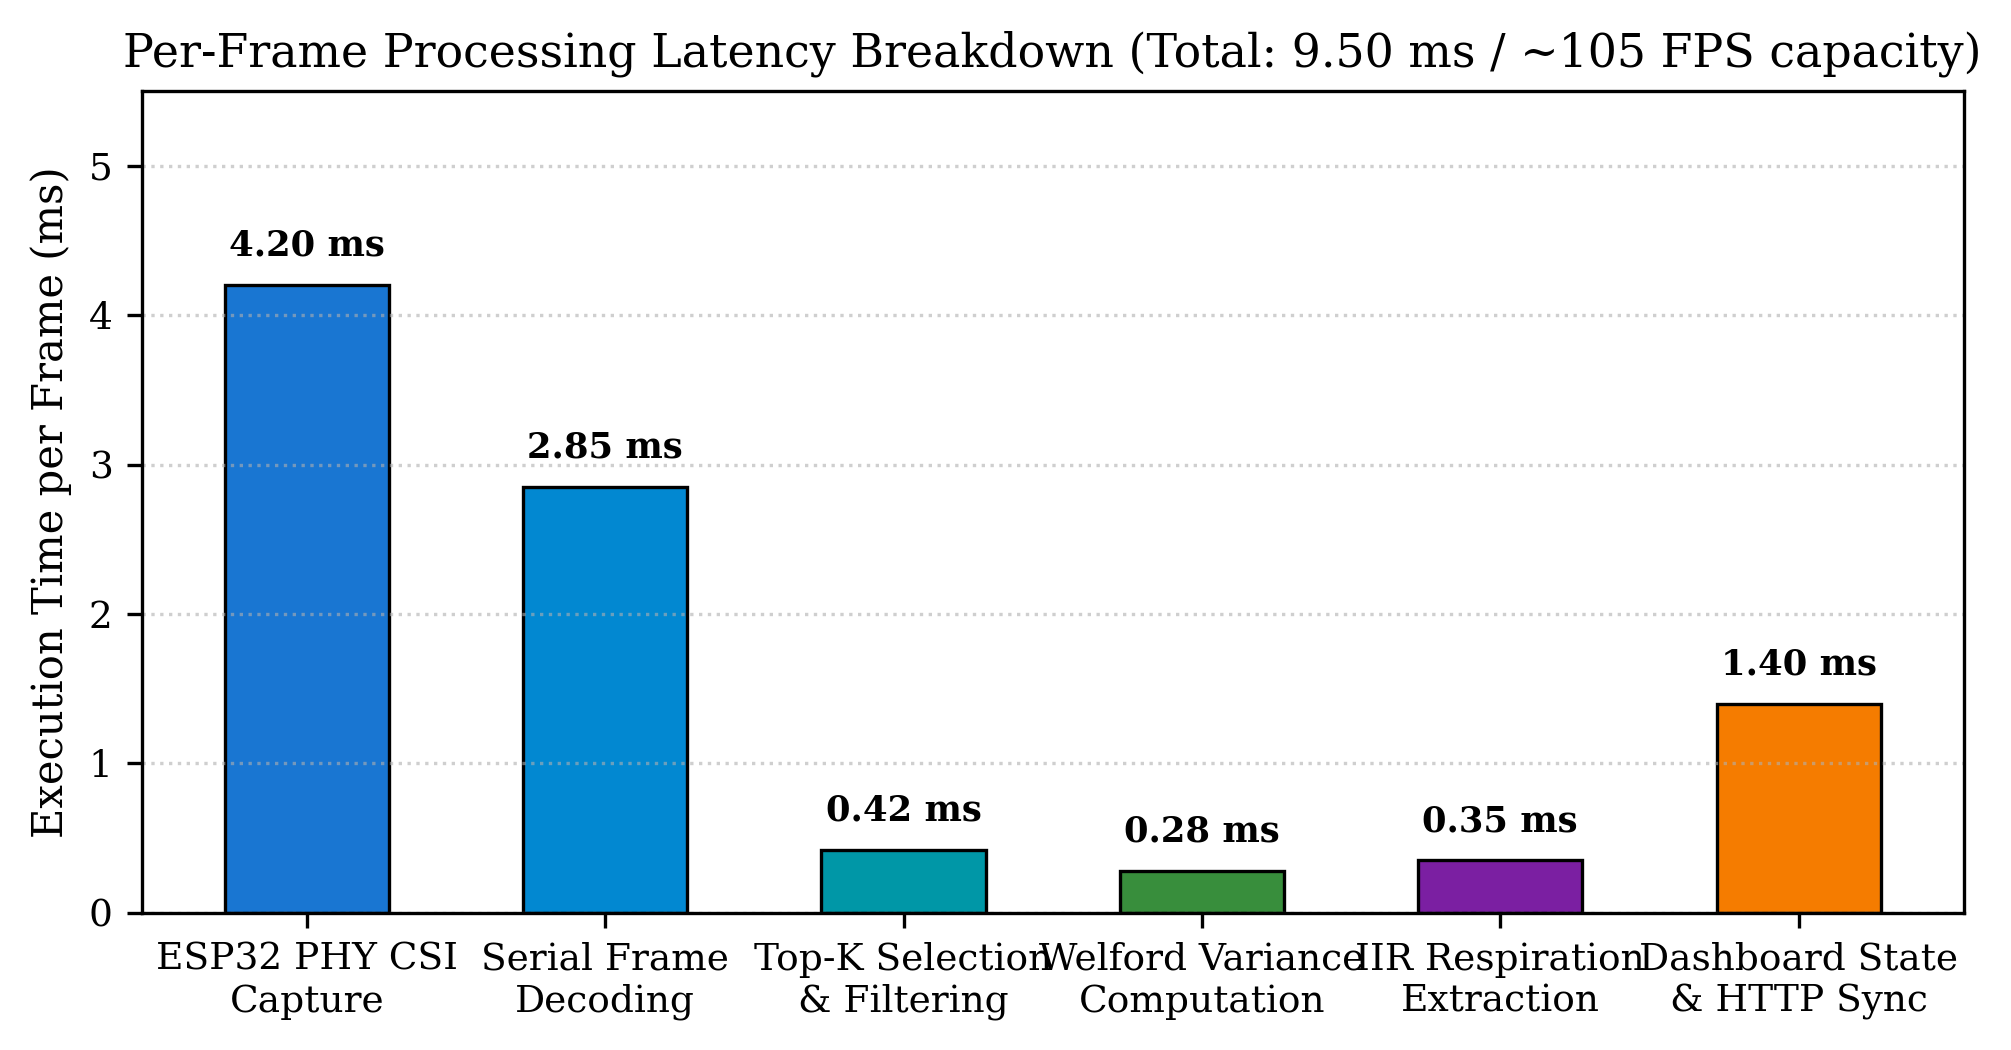
\includegraphics[width=0.85\textwidth]{figures/fig7_latency_edge_breakdown.png}
\caption{Per-frame execution latency breakdown across the complete acquisition, signal processing, and visualization pipeline, demonstrating a total processing time of 9.50~ms per frame.}
\label{fig:latency_breakdown}
\end{figure}
